\documentclass{article}

\usepackage[spanish]{babel}
\usepackage[utf8]{inputenc}
\usepackage{graphicx}

\usepackage[margin=1in]{geometry}
\usepackage{url}

\setlength{\parskip}{\baselineskip}
\setlength{\parindent}{0pt}

\begin{document}

	
\begin{titlepage}

\newcommand{\HRule}{\rule{\linewidth}{0.5mm}} % Defines a new command for the horizontal lines, change thickness here

\center % Center everything on the page
 
%----------------------------------------------------------------------------------------
%	HEADING SECTIONS
%----------------------------------------------------------------------------------------

\textsc{\LARGE Instituto Tecnológico de Costa Rica}\\[1.5cm] % Name of your university/college
\textsc{\Large Escuela de Ingeniería en Computación}\\[0.7cm] % Major heading such as course name
\textsc{\large Maestría en Ciencias de la Computación}\\[0.7cm] % Minor heading such as course title
\textsc{\large Introducción a la Biología Molecular Computacional}\\[0.7cm]

%----------------------------------------------------------------------------------------
%	TITLE SECTION
%----------------------------------------------------------------------------------------

\HRule \\[0.4cm]
{ \huge \bfseries Proyecto \#1: Generador de Mapas Cromosómicos}\\[0.4cm] %
{ \huge \bfseries Reporte Escrito}\\[0.4cm] % Title of your document
\HRule \\[1.5cm]
 
%----------------------------------------------------------------------------------------
%	AUTHOR SECTION
%----------------------------------------------------------------------------------------

\begin{minipage}{0.4\textwidth}
\begin{flushleft} \large
\emph{Autores:}\\
Olger Calderón Achío \linebreak
Wilberth Castro Fuentes \linebreak
Diego Pérez Arroyo 
\end{flushleft}
\end{minipage}
~
\begin{minipage}{0.4\textwidth}
\begin{flushright} \large
\emph{Profesor:} \\
Francisco Torres Rojas, PhD % Supervisor's Name
\end{flushright}
\end{minipage}\\[2cm]

% If you don't want a supervisor, uncomment the two lines below and remove the section above
%\Large \emph{Author:}\\
%John \textsc{Smith}\\[3cm] % Your name

%----------------------------------------------------------------------------------------
%	LOGO SECTION
%----------------------------------------------------------------------------------------


\includegraphics[scale=0.5]{logo_tec.jpg}\\[2cm] % Include a department/university logo - this will require the graphicx package

%----------------------------------------------------------------------------------------
%	DATE SECTION
%----------------------------------------------------------------------------------------

{\large 18 de Abril del 2015}\\ % Date, change the \today to a set date if you want to be precise

%----------------------------------------------------------------------------------------

\vfill % Fill the rest of the page with whitespace

\end{titlepage}

	\tableofcontents
	\pagebreak
	
	\section{Introducción}
	
	El presente documento representa una recopilación de la información más importante concerniente a la implementación del primer proyecto programado del curso. Dicho proyecto se centra en la generación de mapas cromosómicos (o mapas de ligamiento genético) dado que se poseen algunos datos sobres los genes. Dichos mapas representan gráficamente las posiciones relativas entre genes de un mismo cromosoma, y ésto para el biólogo molecular tiene mucha importancia práctica. El proyecto fue implementado en C sobre Linux, más concretamente, Ubuntu.
	
	En la primera sección del documento se analizan conceptos tales como: recombinación de cromosomas, probabilidades de \emph{crossover}, relación entre mapas genéticos y mapas físicos, centimorgans, entre otros. También se adjunta nuestro análisis sobre algunos papers de importancia en el tema. A pesar de que varios investigadores presentaron algoritmos concretos y eficientes para tratar la problemática de generación de mapas, éstos no se ajustaban perfectamente al enunciado del proyecto. Algunos papers presentaban propuestas para encontrar el mejor mapa dado algún criterio previamente escogido, mientras que en nuestro caso, lo que  interesa es poder generar todos los mapas posibles. Así que en este caso nos aventuramos a crear un algoritmo original, no sin tomar antes en cuenta información obtenida de la literatura.
	
	En la segunda parte del documento se profundiza un poco más en la aplicación creada. Primero se mencionan los desafíos técnicos y herramientas utilizadas. Luego se exponen varias imágenes ilustrativas, detallando la funcionalidad lograda en la aplicación. Se finaliza con algunos ejemplos de problemas resueltos por nuestra aplicación, así como con una reflexión de aquellos que transcienden este proyecto, pero que por supuesto tienen un interés en la comunidad científica.
	
	\section{Primera Parte: Acerca de los Mapas Cromosómicos}
	
	\subsection{Algunos conceptos importantes}
	
	Conviene repasar un poco la importancia de los cromosomas, y como el confirmar sus papeles en la herencia causó cierta revolución sobre lo que se pensaba que era un ``gen''. Recopilamos cierta información de \cite{terwilliger1994handbook} y \cite{carrinnes2003handbook}, pero lo que se expone a continuación es nuestra interpretación de los conceptos.
	
	Al principio el concepto de ``gen'' era sumamente abstracto. No se tenía clara su forma, su ubicación, incluso su forma de operar. ¿Había alguna relación entre los distintos genes? ¿O eran totalmente independientes? Con la reivindicación de Gregor Mendel se le dio mucha preponderancia a sus trabajos en la comunidad de biólogos. Mendel afirmaba que los genes actuaban de forma independiente y se mezclaban en las nuevas generaciones de una manera uniforme. Sin embargo en la década de 1910, Thomas Hunt Morgan corroboró la todavía controversial teoría cromosómica Boveri-Sutton. Así quedó claro que los cromosomas controlaban la herencia, y si existía algún lugar ``real'' donde ubicar los genes, era dentro de los ``cuerpos de colores''. Todo esto seguía siendo abstracto, pero abrió la puerta a nuevos marcos del pensamiento.
	
	Con sus trabajos con la mosca de la fruta y los cromosomas sexuales, Morgan también dedujo al observar las proporciones con la que aparecían ciertos fenotipos, que éstos no seguían las leyes Mendelianas al pie de la letra. No parecía que hubiese una independencia real entre algunos grupos de genes. Con esto, Morgan se aventuró a plantear que algunos genes posiblemente estaban ligados. Los genes ligados no seguían los patrones de distribución de las leyes mendelianas, ya que parecían heredarse juntos con más frecuencia. Vienen en paquete se podría decir.
	
	\begin{figure}[h]
		\centering
		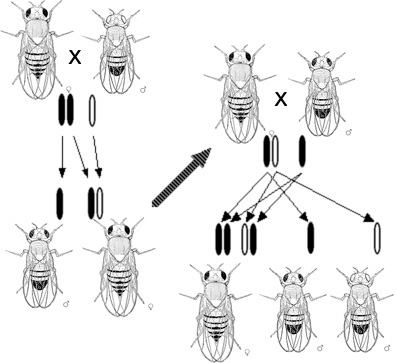
\includegraphics[width=0.5\textwidth]{images/1.jpg}
		\caption{Experimentos de Morgan con la mosca de la fruta. Fuente de imagen: \cite{morgan1919physical}}
		\label{1}
	\end{figure}
	
	
	Hoy día sabemos que este fenómeno tiene que ver con la recombinación de cromosomas (o \emph{crossover} en inglés). Durante la meiosis, porciones de material genético de la madre se mezclan con el material genético del padre, formando cromosomas híbridos. Es una forma de intercambiar material genético entre los seres vivos y de ``sacudirlo'' un poco. Todo ésto juega un papel importante en la evolución.
	
	\begin{figure}[h]
		\centering
		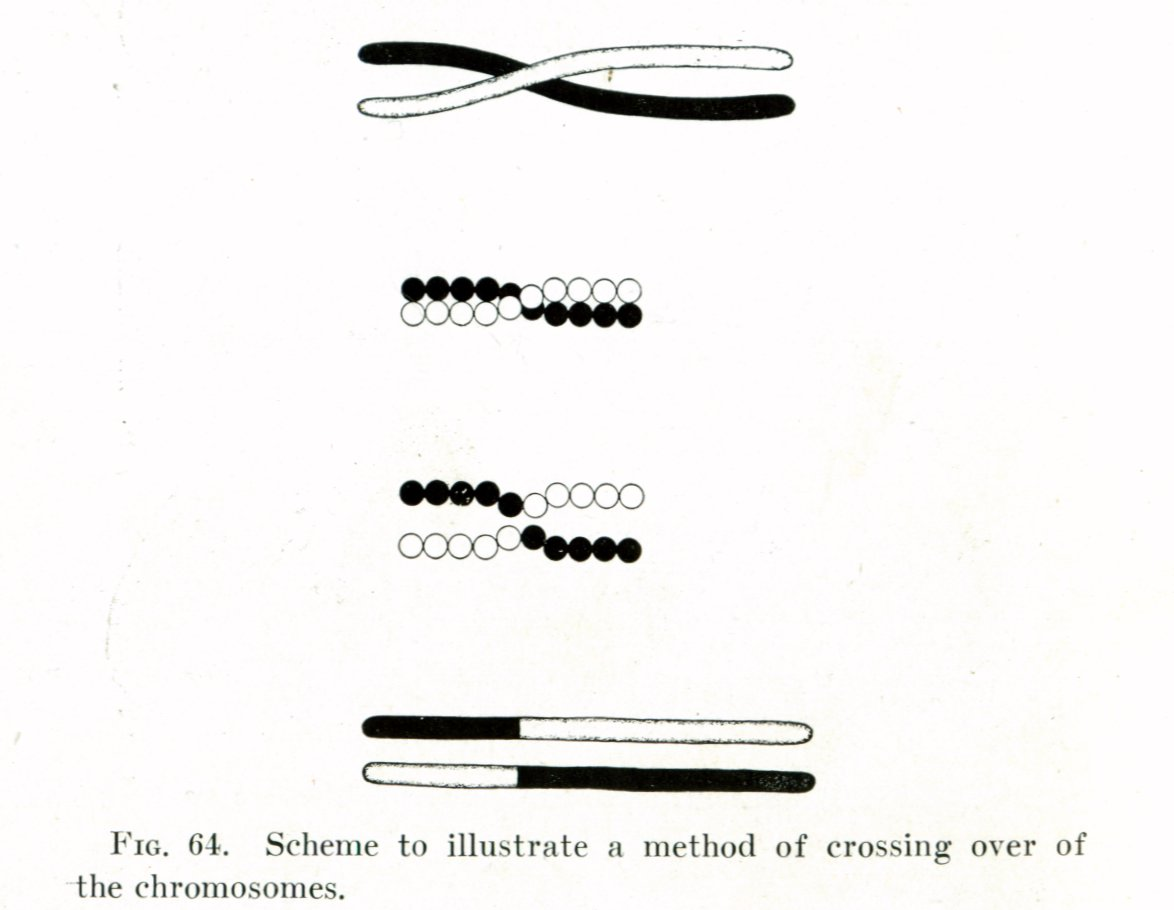
\includegraphics[width=0.5\textwidth]{images/2.jpg}
		\caption{\emph{``Crossover simple''}. Fuente de imagen: \cite{morgan1916critique}}
		\label{2}
	\end{figure}
	
	A muy alto nivel el proceso es como sigue. La meiosis es un tipo de división celular que da paso a la creación de 4 células sexuales o gametos. Cada uno de estos gametos sólo posee una copia de cada cromosoma a diferencia de la mayoría de otras células del cuerpo que poseen dos. En un proceso de meiosis, después de haber ocurrido dos juegos de divisiones, quedan 4 versiones de cada cromosoma que son distribuidas en un gameto cada una. Un cromosoma es idéntico al del padre del individuo, otro es idéntico al de la madre, y los otros dos usualmente se recombinan. En términos muy simplistas, el recombinar dos cromosomas es cortarlos en uno o más puntos, y luego intercambiar segmentos homólogos entre los mismos. Nótese que si todo sale bien, ambos cromosomas recombinados estarán completos después del proceso.
	
	\begin{figure}[h]
		\centering
		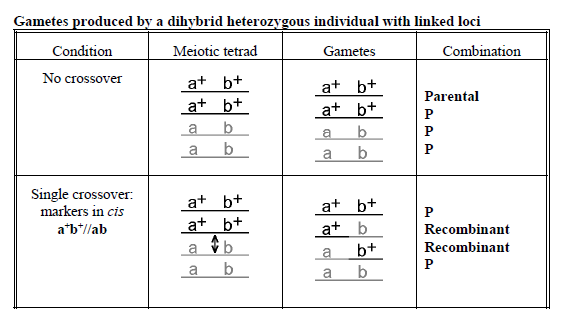
\includegraphics[scale=0.7]{images/3.png}
		\caption{Resultados de meiosis. Fuente de imagen: \cite{carrinnes2003handbook}}
		\label{3}
	\end{figure}
	
	Es un buen momento para definir el concepto de probabilidad de ``crossover'' que es vital para este proyecto. La probabilidad de recombinación entre dos genes es básicamente, la probabilidad de que al escoger un gameto cualquiera, cada gen provenga de un progenitor distinto. En otras palabras y de una forma equivalente, es la probabilidad de que los genes que formaban parte de un mismo cromosoma, sean separados durante la meiosis. 
	
	Sea $P$ una probabilidad de recombinación entre dos genes $G1$ y $G2$, se cumple siempre que $0 \le P \le 0.5$. Esto es sencillo de explicar. Hay dos situaciones posibles. Que los genes sean parte del mismo grupo de ligamiento (en cuyo caso es muy posible que estén en el mismo cromosoma), o bien, que estén en diferentes grupos de ligamiento (diferentes cromosomas). En el último caso, es cuando se deben cumplir las predicciones de Mendel ($P = 0.5$), ya que realmente hay una independencia en la ubicación física de los genes. En caso de que los genes estén ligados, la probabilidad de que sean separados es menor que $0.5$.  
	
	Lo interesante de todo lo anterior es que la probabilidad de recombinación es directamente proporcional a la distancia física entre los genes. Si están más cerca, costará más que haya un corte que los separe. Por eso entre menor sea la probabilidad de ``crossover'' entre dos genes, estos tenderán más a viajar juntos de una generación a otra. A la posición que ocupa un gen en un cromosoma se le llama loci. Si dos genes están tan cerca que cuesta demasiado que se separen se podría decir que están en el mismo loci.
	
	La magia del trabajo de Morgan fue, con base en observaciones de los fenotipos, intuir cuáles eran las probabilidades de ``crossover'' entre los genes. Sin saber nada acerca de la composición química de los genes, sus predicciones fueron de lo más certeras. Uno de sus aprendices, Alfred Henry Sturtevant estudió el primer mapa de ligamiento del cromosoma X de \emph{Drosophila melangaster} \cite{sturtevant1913linear}. Estos mapas son una representación gráfica de la distancia relativa que hay entre los genes, distancias que como se dijo anteriormente son proporcionales a las probabilidades de recombinación entre los genes. La generación de estos mapas son el foco de este proyecto.
	
	Aplicaciones prácticas de crear estos mapas pueden ser: tratar de predecir la posición de un gen responsable de alguna enfermedad, asistir en las mejoras genéticas, descubrir asociaciones entre genes y asistir en la clonación de genes.

	\subsection{Unidades de medida}
	
	En honor al trabajo de Morgan, la principal unidad de medida utilizada en estos mapas es el cM (centimorgan) = 1 unidad de mapa \cite{terwilliger1994handbook}. Un centimorgan equivale a aproximadamente una fracción de recombinación del 1\% o $0.01$. En el presente proyecto, los diagramas de los mapas hacen uso de esta medida para representar que tan ligados están los genes. Un 1 cM corresponde a aproximadamente un millón de pares de bases en los seres humanos \cite{lodish2008molecular}. Este número puede variar de especie a especie.
	
	\subsection{Mapas genéticos y mapas físicos}
	
	Los cM, y en general, los mapas de ligamiento genéticos no son utilizados para medir distancias físicas. Para eso existen los mapas físicos \cite{setubal1997introduction}.
	
	Los primeros mapas genéticos fueron generados experimentando con generaciones sucesivas de organismos y analizando los porcentajes de segregación de ciertas características. En un mapa de ligamiento interesa representar el orden y posiciones de los genes en el cromosoma. Sin embargo no son tan útiles para medir las distancias físicas (pares de bases), ya que si dos genes están demasiado cerca, ocuparán el mismo loci en el mapa.
	
	Los mapas físicos reflejan la distancias reales, y operan a un nivel mayor de detalle. Usualmente se usan otras técnicas distintas para construirlos. Finalmente otro recurso que opera a un nivel mayor de detalle sería la secuenciación \cite{setubal1997introduction}.
	
	\subsection{Gregor Mendel}
	
	
	
	\subsection{Literatura consultada}
	El paper de Stutervant y el de Morgan, más el primero que el segundo, nos sientan las bases de los mapas cromosómicos de genes ligados. Nos explica cómo se llego a la idea de que la probabilidad de crossover estaba relacionada con la distancia de los genes en los cromosomas.  Morgan define conceptos que son fundamentales tener claros; estos dos papers son la base que había que tener clara antes de si quiera tratar de pensar en la solución al problema. Sin embargo, una vez que se han leído y entendido, para los efectos del proyecto, no proporcionan mucha ayuda. Reafirma la teoría vista en clase. No trata temas como probabilidades faltantes, mapeo de genes no ligados y otros detalles.

	El paper de más ayuda fue el llamado “Efficient and accurate construction of genetic linkage maps from noisy and missing genotyping data”. Una vez leído el título pensamos que iba a resolver todos nuestras dudas, porque parece ser justo el mismo tema del proyecto: construcción eficiente de mapas de ligamiento, manejo de datos faltantes. Empero, en realidad el problema que trata es distinto. El objetivo de los autores es construir el mejor mapa de ligamiento posible de forma eficiente. Parten de una población de individuos, en los cuales hay genes que se expresan de una u otra forma. Estiman la probabilidad de crossover entre genes al determinar el número de veces que un gen se expresa de la misma forma en todos los individuos.

	Una vez determinadas las probabilidades de crossover entre los genes entonces pareciera encontrarse en el punto inicial de nuestro proyecto. El siguiente paso del paper es hacer clustering para determinar los grupos de ligamiento de genes. Es importante destacar en este punto que gracias a lo leído nos dimos cuenta que la probabilidad de crossover entre 2 genes ligados está entre [0 – 0.5] esto porque si la probabilidad es de 0.5 significa que los genes se expresan independientemente y por lo general estarían ubicados en diferentes cromosomas. Del paper entendimos que básicamente se determinan los grupos de genes ligados al realizar un recorrido en profundidad del grafo (matriz inicial del proyecto) ignorando las aristas con valor a 0.5 o muy cercanas a dicho valor. El resultado son componentes conexos del grafo original, cada uno de ellos es un grupo de ligamiento.

	Es en este punto en que el paper nos deja de ser útil. Los siguientes pasos se centran en determinar el orden óptimo de los genes para que el mapa sea de menor tamaño. Varios métodos son presentados e incluso uno propio por parte de los autores. Mas, para nuestros efectos no eran de ayuda pues el problema del proyecto es generar todos los posibles mapas no sólo el óptimo. De igual forma cuando se  trataba sobre datos faltantes el paper no nos fue de utilidad porque de nuevo el enfoque de los autores difiere del nuestro.

	El paper “Efficient and accurate construction of genetic linkage maps from noisy and missing genotyping data” es el mismo que el anterior sólo que en una edición un año después por parte de los mismos autores. No nos aporta nada que no lo haya hecho su predecesor.

	
	
	\section{Segunda Parte: Aplicación Creada}
	
	\subsection{Detalles técnicos de implementación}
	
	Nos basamos principalmente en las herramientas de desarrollo de GNOME y en la cadena de herramientas de GNU. De estas últimas podemos citar el compilador gcc, la herramienta de construcción make y el GNU Build System (autotools). Por el lado de GNOME, se utilizó el IDE Anjuta, el diseñador de interfaces gráficas Glade, y la colección de componentes gráficos GTK+3.0.
	
	Una pregunta importante de implementación fue: ¿Cómo graficamos los mapas cromosómicos?. Contemplamos varias opciones entre ellas: graficar los mapas usando primitivas de Cairo, usando el canvas Clutter, e incluso, openGL. Realizar los mapas usando Cairo parecía caro y tal vez no se iba a lograr un resultado sorprendente. Por otra parte Clutter parecía algo complejo y tal vez mucho más de lo necesario. Así que se optó por investigar si existía algún canvas de dibujo específico para bioinformáticos. Para nuestro asombro encontramos Genome Tools (\url{http://genometools.org/}), que es posiblemente el marco de trabajo más importante para bioinformáticos que desean hacer aplicaciones en C. Dicho proyecto, no es solamente una biblioteca, sino también un conjunto de aplicaciones basadas sobre la misma. Para nuestros propósitos nos interesó usar \emph{Annotation Sketch}, un conjunto de clases y módulos con la capacidad de crear diagramas para representar información genómica. La biblioteca es muy personalizable, y claramente cumplía con nuestros requerimientos. En el fondo \emph{Annotation Sketch} hace llamados a las primitivas de Cairo. Lo único que se debe proveer es un grafo de objetos representando la información de los genes que se desea graficar y la relación entre ellos. La información no está limitada a genes, se puede incluir también: cromosomas, exones, intrones, segmentos de ARN mensajero, entre otros. A pesar de ello, la herramienta estaba más orientada a graficar mapas físicos (en términos de pares de bases), por lo que requirió cierto trabajo el ajustar los gráficos para que pareciesen más mapas de ligamiento de genes. Para una mayor información sobre las ventajas de usar Genome Tools en términos de eficiencia, y para una introducción a sus representaciones se puede consultar \cite{gremme2013genometools}.
	
	% Wilberth, agregar algunos detalles sobre la implementación del grid dinámico.
	
	% Diego agregar detalles sobre el algoritmo implementado.
	
	\subsection{Imágenes ilustrativas de la aplicación}
	
	
	\subsection{Problemas resueltos por nuestra aplicación}
	
	
	\subsection{Problemas que trascienden el alcance del proyecto}
	
	Nuestro proyecto hace una serie de suposiciones que simplifica un poco su alcance. Por ejemplo los eventos de recombinación son simples. Sólo hay un intercambio en un evento de meiosis. Cuando hay más de un ``crossover'' en el mismo evento meiótico, puede que haya que transformar las probabilidades de recombinación a una cantidad de cM distinta. Funciones que realizan estas transformaciones son las de Haldane y Kosambi. Por ejemplo la función de Haldane sobre una probabilidad de $0.27$, retorna 39 cM, mientras que la de Kosambi 30cM \cite{terwilliger1994handbook}.
	
	El tema se puede tornar tan complicado como se quiera, y hay aspectos que se vuelven más difíciles de modelar. Entre algunos de estos aspectos se puede mencionar las probabilidades de mutación y desequilibrio de ligamiento. El paquete LINKAGE contempla mucho de estos problemas y más \cite{terwilliger1994handbook}.
	
	\section{Conclusiones}
	
	El proyecto fue sumamente provechoso, desde muchos puntos de vista. Por un lado se recopiló información sobre temas de biología, como es el de los mapas de ligamiento genéticos. Se comprendió su importancia práctica y repercusiones en el campo de la Biología Molecular.
	
	Desde el punto de vista algorítmico tan bien fue muy valioso. Nos dimos cuenta como en efecto, muchos problemas de la naturaleza pueden modelarse en términos de árboles y grafos. A veces resulta sorprendente como conceptos como árboles de expansión minimal y componentes conexos representan de forma muy aproximada algún concepto del problema que se trata. Se tuvieron discusiones y disyuntivas sobre cuál era la mejor forma de atacar el problema. Como se mencionó en la introducción del documento, al final se optó por la creatividad del grupo para la implementación del algoritmo, aunque esto representara cambiar ligeramente la forma de modelar y tratar el problema. Toda esta experiencia estimula el analizar los algoritmos más detenidamente.
	
	Por el lado de programación, nos adentramos de nuevo al mundo de programación en C, recordando así el potencial del lenguaje. Al encontrar una biblioteca como Genome Tools, nos dimos cuenta de que existe una comunidad que realiza aplicaciones para bioinformáticos. Ellos siguen estándares y apuestan en C como en el lenguaje apropiado para la implementación. No está de más conocer la existencia de tan útil proyecto. Por otra parte se sacó provecho de las herramientas libres de GNOME, donde GTK+ resalta con un kit muy completo de componentes gráficos.
	
	\bibliographystyle{plain}
	\bibliography{refs}
	
\end{document}